\section{Results}\label{sec:results}

\subsection{Retrieval}\label{sec:res-retrieval}
Table~\ref{tab:retrieval} gives retrieval quality on the generation queries, and Table~\ref{tab:ci} gives the intervals. On NQ, the dense encoders differed widely. MiniLM-L6 reached \ev{HIT.nq.R1} and e5-base-v2 \ev{HIT.nq.R5}; bge-large (\ev{HIT.nq.R4}) came second. Qwen3-Embedding-0.6B (\ev{HIT.nq.R6}) placed between bge-small and bge-base. BM25 reached \ev{HIT.nq.R0}. On HotpotQA, Hit@5 nearly saturated: all dense encoders except MiniLM-L6 scored between \ev{HIT.hp.R6} and \ev{HIT.hp.R4}, against \ev{HIT.hp.R1} for MiniLM-L6 and \ev{HIT.hp.R0} for BM25. The stricter Both@5 separated them more clearly: bge-large found both supporting passages for \ev{BOTH.hp.R4} of the questions, e5-base-v2 for \ev{BOTH.hp.R5}, Qwen3-Embedding-0.6B for \ev{BOTH.hp.R6} and MiniLM-L6 for \ev{BOTH.hp.R1}. Table~\ref{tab:retrieval} also gives Hit@1, Hit@10, nDCG@10 and MRR@10, and Fig.~\ref{fig:retrieval} shows the main metrics with their intervals. On NQ, nDCG@10 ordered the retrievers as Hit@5 did, from \ev{RET.nq.ndcg10.R0} for BM25 and \ev{RET.nq.ndcg10.R1} for MiniLM-L6 to \ev{RET.nq.ndcg10.R5} for e5-base-v2. On HotpotQA, nDCG@10 ranged from \ev{RET.hp.ndcg10.R1} (MiniLM-L6) to \ev{RET.hp.ndcg10.R4} (bge-large).

\begin{figure}[t]
\centering
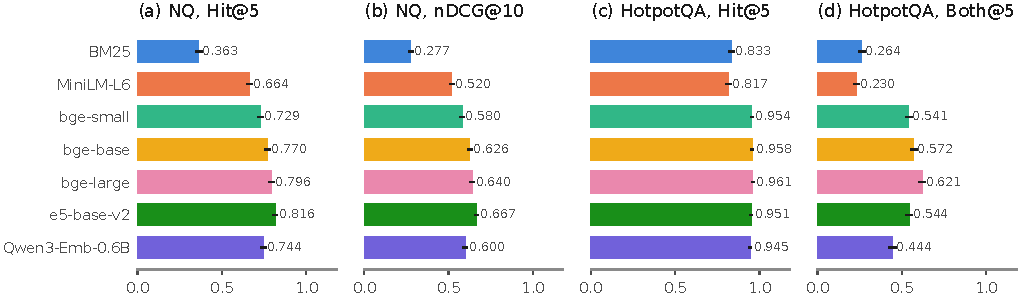
\includegraphics[width=\linewidth]{figs/fig9_retrieval.pdf}
\caption{Retrieval quality on the generation queries with 95\% bootstrap intervals: NQ Hit@5 and nDCG@10 (2,255 queries), HotpotQA Hit@5 and Both@5 (2,000 queries).}
\label{fig:retrieval}
\end{figure}

\begin{table*}[t]
\centering
\footnotesize
\setlength{\tabcolsep}{3.5pt}
\caption{Retrieval quality on the generation queries of each dataset (300,000-passage sub-corpora, exact search).}
\label{tab:retrieval}
\begin{tabular}{lcccccccccc}
\toprule
 & \multicolumn{5}{c}{NQ (2,255 queries)} & \multicolumn{5}{c}{HotpotQA (2,000 queries)} \\ \cmidrule(lr){2-6}\cmidrule(lr){7-11}
Retriever & Hit@1 & Hit@5 & Hit@10 & nDCG@10 & MRR@10 & Hit@1 & Hit@5 & Both@5 & nDCG@10 & MRR@10 \\
\midrule
BM25 & 0.150 & 0.363 & 0.472 & 0.277 & 0.243 & 0.666 & 0.833 & 0.264 & 0.578 & 0.740 \\
MiniLM-L6 & 0.316 & 0.664 & 0.792 & 0.520 & 0.462 & 0.623 & 0.817 & 0.230 & 0.549 & 0.708 \\
bge-small & 0.375 & 0.729 & 0.843 & 0.580 & 0.526 & 0.812 & 0.954 & 0.541 & 0.756 & 0.874 \\
bge-base & 0.421 & 0.770 & 0.882 & 0.626 & 0.570 & 0.836 & 0.958 & 0.572 & 0.777 & 0.888 \\
bge-large & 0.430 & 0.796 & 0.888 & 0.640 & 0.584 & 0.846 & 0.961 & 0.621 & 0.797 & 0.897 \\
e5-base-v2 & 0.458 & 0.816 & 0.906 & 0.667 & 0.612 & 0.799 & 0.951 & 0.544 & 0.751 & 0.864 \\
Qwen3-Emb-0.6B & 0.400 & 0.744 & 0.843 & 0.600 & 0.547 & 0.810 & 0.945 & 0.444 & 0.717 & 0.868 \\
\bottomrule
\end{tabular}
\par\smallskip\parbox{\linewidth}{\footnotesize NQ intervals for Hit@5 and nDCG@10 are in Table~\ref{tab:ci} and Fig.~\ref{fig:retrieval}. Both@5: both gold passages in the top five.}
\end{table*}


\subsection{Answer gains and transfer ratios (RQ1)}\label{sec:res-transfer}
Table~\ref{tab:main} gives EM for every cell with its two reference conditions, and Fig.~\ref{fig:hitem} plots EM against Hit@5. Retrieval closed only part of the gap between the closed-book and gold-passage conditions. With Qwen on NQ, closed-book EM was \ev{EM.qnq.CB}, gold passages gave \ev{EM.qnq.GOLD}, and the best retriever, e5-base-v2, gave \ev{EM.qnq.R5}. With Llama on NQ the best retriever was bge-base (\ev{EM.lnq.R3}) against a gold-passage reference of \ev{EM.lnq.GOLD}. On HotpotQA, bge-large gave the highest EM for both readers (\ev{EM.qhp.R4} and \ev{EM.lhp.R4}), against gold-passage references of \ev{EM.qhp.GOLD} and \ev{EM.lhp.GOLD}.

\begin{figure}[t]
\centering
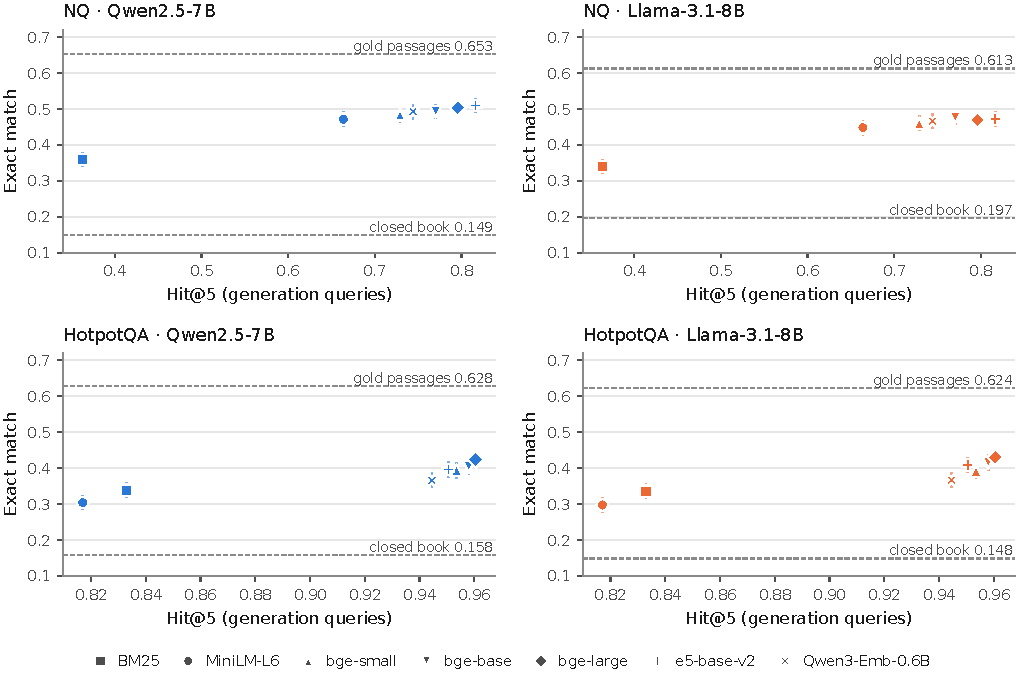
\includegraphics[width=\linewidth]{figs/fig2_hit_vs_em.pdf}
\caption{Exact match against Hit@5 for each retriever in the four reader--dataset cells. Vertical bars are 95\% bootstrap intervals for EM. Dashed lines mark the closed-book and gold-passage reference conditions. Note the different Hit@5 ranges of the two datasets.}
\label{fig:hitem}
\end{figure}

Table~\ref{tab:transfer} and Fig.~\ref{fig:transfer} give the transfer ratios. On NQ, the five dense encoders had ratios between \ev{T.lnq.R4} (bge-large and e5-base-v2 with Llama) and \ev{T.lnq.R3} (bge-base with Llama). With Qwen, e5-base-v2 gained \ev{DH.qnq.R5} in Hit@5 over MiniLM-L6 but only \ev{DE.qnq.R5} in EM, a ratio of \ev{T.qnq.R5} \ev{T.qnq.R5.ci}. The intervals for bge-small included zero in both NQ cells (Qwen \ev{T.qnq.R2.ci}, Llama \ev{T.lnq.R2.ci}), so its NQ ratio is uncertain in sign. The largest NQ upper bound was \ev{V5.nq.ubmax} (Qwen3-Embedding-0.6B with Qwen). BM25 retrieved worse than MiniLM-L6 on NQ, so its ratio (\ev{T.qnq.R0} with Qwen) relates an EM loss to a Hit@5 loss.

With Hit@5 as the denominator, the HotpotQA ratios were larger for every encoder and reader, from \ev{T.qhp.R6} (Qwen3-Embedding-0.6B with Qwen) to \ev{T.lhp.R4} (bge-large with Llama). With Qwen, every upper bound stayed below 1, the largest being \ev{T.qhp.R4.hi3} for bge-large. With Llama, the bounds were \ev{T.lhp.R3.hi3} for bge-base, \ev{T.lhp.R5.hi3} for e5-base-v2 and \ev{T.lhp.R4.hi3} for bge-large, so the P1 criterion (every upper bound below 1) was met in the two new NQ and Qwen--HotpotQA cells and not met in the Llama--HotpotQA cell (Table~\ref{tab:predictions}). The BM25 ratio was not estimable on HotpotQA, because BM25 and MiniLM-L6 differed by only \ev{DH.qhp.R0} in Hit@5.

\begin{figure}[t]
\centering
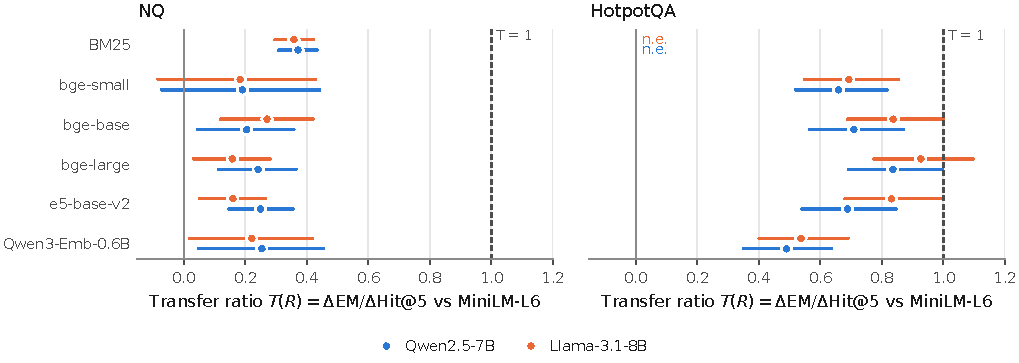
\includegraphics[width=\linewidth]{figs/fig1_transfer_ratios.pdf}
\caption{Transfer ratio $T(R)=\Delta\mathrm{EM}/\Delta\mathrm{Hit@5}$ against MiniLM-L6 with 95\% bootstrap intervals. The dashed line marks $T=1$, a reference point. n.e.: not estimable under the reporting rule.}
\label{fig:transfer}
\end{figure}

\begin{table*}[t]
\centering
\small
\caption{Retrieval (Hit@5) and answer quality (exact match) for each reader and dataset. Hit@5 is computed on the generation queries; 95\% bootstrap intervals are in Table~\ref{tab:ci}.}
\label{tab:main}
\begin{tabular}{lrrrrrrrr}
\toprule
 & \multicolumn{4}{c}{NQ (2,255 queries)} & \multicolumn{4}{c}{HotpotQA (2,000 queries)} \\ \cmidrule(lr){2-5}\cmidrule(lr){6-9} & \multicolumn{2}{c}{Qwen} & \multicolumn{2}{c}{Llama} & \multicolumn{2}{c}{Qwen} & \multicolumn{2}{c}{Llama} \\ \cmidrule(lr){2-3}\cmidrule(lr){4-5}\cmidrule(lr){6-7}\cmidrule(lr){8-9}
Retriever & Hit@5 & EM & Hit@5 & EM & Hit@5 & EM & Hit@5 & EM \\
\midrule
BM25 & 0.363 & 0.360 & 0.363 & 0.340 & 0.833 & 0.339 & 0.833 & 0.336 \\
MiniLM-L6 & 0.664 & 0.471 & 0.664 & 0.448 & 0.817 & 0.304 & 0.817 & 0.297 \\
bge-small & 0.729 & 0.484 & 0.729 & 0.460 & 0.954 & 0.394 & 0.954 & 0.392 \\
bge-base & 0.770 & 0.493 & 0.770 & 0.477 & 0.958 & 0.404 & 0.958 & 0.415 \\
bge-large & 0.796 & 0.503 & 0.796 & 0.469 & 0.961 & 0.424 & 0.961 & 0.430 \\
e5-base-v2 & 0.816 & 0.510 & 0.816 & 0.472 & 0.951 & 0.396 & 0.951 & 0.408 \\
Qwen3-Emb-0.6B & 0.744 & 0.492 & 0.744 & 0.466 & 0.945 & 0.366 & 0.945 & 0.366 \\
Closed book & -- & 0.149 & -- & 0.197 & -- & 0.158 & -- & 0.148 \\
Gold passages & -- & 0.653 & -- & 0.613 & -- & 0.628 & -- & 0.624 \\
\bottomrule
\end{tabular}
\end{table*}

\begin{table*}[t]
\centering
\small
\caption{Transfer ratio $T(R)=\Delta\mathrm{EM}/\Delta\mathrm{Hit@5}$ relative to MiniLM-L6, with 95\% bootstrap intervals.}
\label{tab:transfer}
\begin{tabular}{lcccc}
\toprule
Retriever & NQ Qwen & NQ Llama & HotpotQA Qwen & HotpotQA Llama \\
\midrule
BM25 & 0.37 [0.31, 0.43] & 0.36 [0.30, 0.42] & n.e. & n.e. \\
bge-small & 0.19 [$-$0.07, 0.44] & 0.18 [$-$0.08, 0.43] & 0.66 [0.52, 0.82] & 0.69 [0.55, 0.85] \\
bge-base & 0.20 [0.04, 0.36] & 0.27 [0.12, 0.42] & 0.71 [0.57, 0.87] & 0.84 [0.69, 1.00] \\
bge-large & 0.24 [0.11, 0.36] & 0.16 [0.03, 0.28] & 0.84 [0.69, 1.00] & 0.93 [0.78, 1.10] \\
e5-base-v2 & 0.25 [0.15, 0.36] & 0.16 [0.05, 0.26] & 0.69 [0.54, 0.85] & 0.83 [0.68, 1.00] \\
Qwen3-Emb-0.6B & 0.25 [0.05, 0.45] & 0.22 [0.02, 0.42] & 0.49 [0.35, 0.64] & 0.54 [0.40, 0.69] \\
\bottomrule
\end{tabular}
\par\smallskip\parbox{\linewidth}{\footnotesize n.e.: not estimable under the pre-registered rule ($|\Delta\mathrm{Hit@5}|\le 2$ points or not significant after Holm). BM25 on NQ retrieves worse than MiniLM-L6, so its ratio describes a loss.}
\end{table*}


\subsection{How stable are the ratios?}\label{sec:res-sens}
Table~\ref{tab:sensitivity} repeats the dense-encoder ratios under other answer metrics, another baseline, another retrieval metric and other numbers of passages. Only the top row is the registered analysis.

On NQ, one pattern held in every row read at $k\geq 3$: each ratio and each upper bound stayed well below 1. With token F1 the NQ ratios were \ev{V5.f1.nq}, with answer containment \ev{V5.ac.nq}, and against BM25 instead of MiniLM-L6 \ev{V4.b0.nq.min}--\ev{V4.b0.nq.max}; the largest upper bound over these rows was \ev{V5.nq.allub}. The size of the ratio was not stable, however. It fell with the number of passages read: \ev{V5.k1.range} at $k=1$, \ev{V5.k3.range} at $k=3$ and \ev{V5.k10.range} at $k=10$ (Qwen; exploratory, Hit@$k$ matched to $k$). At $k=1$ the largest upper bound was \ev{V5.k1.ubmax}.

On HotpotQA, the size of the ratio depended mainly on the retrieval metric. With Both@5 instead of Hit@5 as the denominator, the dense-encoder ratios were \ev{V4.both.hp.min}--\ev{V4.both.hp.max} for both readers, close to the NQ ratios against BM25, and Qwen3-Embedding-0.6B no longer stood apart. Against BM25 with Hit@5, the HotpotQA ratios were \ev{V4.b0.hp.min}--\ev{V4.b0.hp.max}; they exceeded the NQ ratios in \ev{V4.b0.hpgt} of 10 encoder--reader pairs, the exceptions being Qwen3-Embedding-0.6B (\ev{V4.b0.qwen_hp.R6} and \ev{V4.b0.llama_hp.R6} against \ev{V4.b0.qwen_nq.R6} and \ev{V4.b0.llama_nq.R6}). Under F1, the Llama ratio of bge-large was \ev{TF.lhp.R4} \ev{TF.lhp.R4.ci}, so full transfer cannot be ruled out for that encoder when it is measured with Hit@5.

The stable finding is therefore that, with three to ten passages read ($k$ = 3, 5 and 10), a Hit@5 gain over a small encoder bought a much smaller EM gain on NQ. The exact ratio depends on the baseline, the answer metric and $k$, and the larger HotpotQA ratios depend on scoring retrieval by any rather than all supporting passages.

\begin{table*}[t]
\centering
\small
\caption{Sensitivity of the dense-encoder transfer ratios (range over five encoders and both readers unless stated). All rows except the top one are secondary or post hoc.}
\label{tab:sensitivity}
\begin{tabular}{lcccc}
\toprule
Answer metric, retrieval metric, baseline & NQ ratios & NQ max. upper & HotpotQA ratios & HotpotQA max. upper \\
\midrule
EM (primary), Hit@5, MiniLM-L6 & 0.16--0.27 & 0.45 & 0.49--0.93 & 1.10 \\
token F1, Hit@5, MiniLM-L6 & 0.23--0.33 & 0.49 & 0.52--1.10 & 1.28 \\
answer containment, Hit@5, MiniLM-L6 & 0.27--0.39 & 0.60 & 0.49--1.01 & 1.18 \\
EM, Hit@5, BM25 & 0.29--0.35 & 0.40 & 0.25--0.75 & 0.92 \\
EM, Both@5, MiniLM-L6 & -- & -- & 0.29--0.35 & 0.41 \\
EM, Hit@$k$ at $k=1$, MiniLM-L6 (Qwen) & 0.41--0.83 & 1.22 & -- & -- \\
EM, Hit@$k$ at $k=3$, MiniLM-L6 (Qwen) & 0.32--0.37 & 0.59 & -- & -- \\
EM, Hit@$k$ at $k=10$, MiniLM-L6 (Qwen) & 0.05--0.19 & 0.42 & -- & -- \\
\bottomrule
\end{tabular}
\par\smallskip\parbox{\linewidth}{\footnotesize Max. upper: largest upper 95\% bootstrap bound in the row. The $k$ rows match Hit@$k$ to the $k$ passages read (Qwen reader, NQ only; exploratory, without the reporting rule).}
\end{table*}


\subsection{Do the NQ ratios hold on the full corpus?}\label{sec:res-full}
All results so far use the 300,000-passage sub-corpus, which favours the dense encoders relative to BM25. In Phase~3 both readers answered the NQ generation queries from retrieval on the full corpus of \ev{V6.enc.rows} passages (Table~\ref{tab:fullreader} and Fig.~\ref{fig:fulltransfer}). On the full corpus the dense encoders lost \ev{V6.dHit.dense.abs} in Hit@5 and \ev{V6.dEM.dense.abs} in EM (all Holm-adjusted $p\le$ \ev{V6.dEM.dense.pmax}). BM25 kept its Hit@5, and its EM changed by no detectable amount (\ev{V6.dEM.R0}; $p\ge$ \ev{V6.dEM.R0.pmin}).

The transfer ratios hardly moved. With e5-base-v2, $T$ was \ev{V6.T3.q.R5} \ev{V6.T.q.R5.ci} with Qwen, inside its sub-corpus interval \ev{V6.P8.q.sub}, and \ev{V6.T3.l.R5} \ev{V6.T.l.R5.ci} with Llama, inside \ev{V6.P8.l.sub}. The paired differences from the sub-corpus ratios were \ev{V6.dT.q} \ev{V6.dT.q.ci} and \ev{V6.dT.l} \ev{V6.dT.l.ci}. The bge-small ratios were \ev{V6.T.q.R2} \ev{V6.T.q.R2.ci} and \ev{V6.T.l.R2} \ev{V6.T.l.R2.ci}; as on the sub-corpus, their intervals included zero. Every dense upper bound stayed below 1 (largest \ev{V6.T.ubmax}), so P7 and P8 were met for both readers. Against BM25, the ratios of bge-small and e5-base-v2 were \ev{V6.b0.full} on the full corpus and \ev{V6.b0.sub} on the sub-corpus.

The query-level accounting also kept its shape. Queries that moved from miss to hit contributed \ev{V6.tr.misshit.contrib} to the EM gain, those that hit under both retrievers \ev{V6.tr.hithit.contrib} (interval below zero in \ev{V6.tr.hithit.neg} of 4 encoder--reader pairs) and those that lost their hit \ev{V6.tr.hitmiss.contrib}. In a comparison that was not pre-specified, the full corpus cost the three dense encoders \ev{V6.lossratio} EM points per Hit@5 point lost, about the size of the transfer ratios themselves. At most \ev{V6.unparsed.max} of the full-corpus outputs could not be parsed.

\begin{figure}[t]
\centering
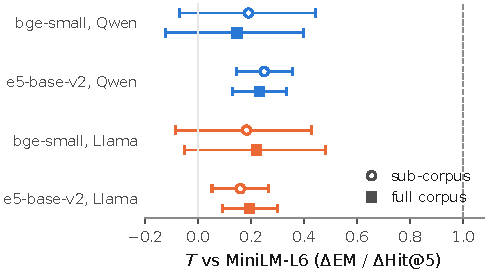
\includegraphics[width=0.75\linewidth]{figs/fig13_fullcorpus_T.pdf}
\caption{NQ transfer ratios against MiniLM-L6 on the sub-corpus (open circles) and on the full corpus (filled squares), with 95\% bootstrap intervals; 2,255 queries, $k=5$. The dashed line marks $T=1$.}
\label{fig:fulltransfer}
\end{figure}

\begin{table*}[t]
\centering
\footnotesize
\caption{NQ readers on the 300,000-passage sub-corpus and on the full 2,681,468-passage corpus (Phase 3), 2,255 generation queries, $k=5$. Intervals are 95\% bootstrap intervals.}
\label{tab:fullreader}
\begin{tabular}{lccccccll}
\toprule
& \multicolumn{2}{c}{Hit@5} & \multicolumn{2}{c}{EM} & & & \multicolumn{2}{c}{$T$ vs MiniLM-L6 [95\% CI]} \\ \cmidrule(lr){2-3}\cmidrule(lr){4-5}\cmidrule(lr){8-9} Retriever & sub & full & sub & full & $\Delta$EM full$-$sub & $p_\text{Holm}$ & sub & full \\
\midrule
\multicolumn{9}{l}{\textit{Qwen2.5-7B}} \\
BM25 & 0.363 & 0.364 & 0.360 & 0.358 & \ensuremath{-}0.001 & 0.798 & 0.37 [0.31, 0.43] & 0.44 [0.35, 0.53] \\
MiniLM-L6 & 0.664 & 0.564 & 0.471 & 0.446 & \ensuremath{-}0.025 & $<$0.001 & -- & -- \\
bge-small & 0.729 & 0.630 & 0.484 & 0.456 & \ensuremath{-}0.028 & $<$0.001 & 0.19 [\ensuremath{-}0.07, 0.44] & 0.15 [\ensuremath{-}0.12, 0.40] \\
e5-base-v2 & 0.816 & 0.728 & 0.510 & 0.484 & \ensuremath{-}0.025 & $<$0.001 & 0.25 [0.15, 0.36] & 0.23 [0.13, 0.33] \\
\midrule
\multicolumn{9}{l}{\textit{Llama-3.1-8B}} \\
BM25 & 0.363 & 0.364 & 0.340 & 0.335 & \ensuremath{-}0.005 & 0.155 & 0.36 [0.30, 0.42] & 0.44 [0.34, 0.54] \\
MiniLM-L6 & 0.664 & 0.564 & 0.448 & 0.423 & \ensuremath{-}0.025 & $<$0.001 & -- & -- \\
bge-small & 0.729 & 0.630 & 0.460 & 0.437 & \ensuremath{-}0.023 & 0.002 & 0.18 [\ensuremath{-}0.08, 0.43] & 0.22 [\ensuremath{-}0.05, 0.48] \\
e5-base-v2 & 0.816 & 0.728 & 0.472 & 0.455 & \ensuremath{-}0.018 & 0.014 & 0.16 [0.05, 0.26] & 0.20 [0.09, 0.30] \\
\bottomrule
\end{tabular}
\par\smallskip\parbox{\linewidth}{\footnotesize Sub-corpus values are those of Table~\ref{tab:transfer}. $\Delta$EM: paired difference full $-$ sub (intervals in the repository), exact McNemar test, Holm over the four retrievers per reader. Full-corpus ratios use the reporting rule with Holm over the six pairs among the four retrievers. BM25's ratio relates an EM loss to a Hit@5 loss.}
\end{table*}


\subsection{Where the gain sits}\label{sec:res-decomp}
\paragraph{Query-level accounting}
Table~\ref{tab:transitions} groups the queries by their Hit@5 under MiniLM-L6 and under each dense encoder (per-encoder values with intervals in Table~\ref{tab:transdetail}). On NQ, \ev{V5.tr.nq.misshit.share} of the queries moved from miss to hit. Their EM rose by \ev{V5.tr.nq.misshit.within} within the group, from a MiniLM-L6 level of \ev{V5.tr.nq.misshit.embase}: many of these ``misses'' had already been answered correctly. This group contributed \ev{V5.tr.nq.misshit.contrib} to the EM gain. Two groups gave part of it back. The \ev{V5.tr.nq.hithit.share} of queries that hit under both retrievers contributed \ev{V5.tr.nq.hithit.contrib} (interval below zero in \ev{V5.tr.nq.hithit.neg} of 10 encoder--reader pairs), and the \ev{V5.tr.nq.hitmiss.share} that lost their hit contributed \ev{V5.tr.nq.hitmiss.contrib} (below zero in \ev{V5.tr.nq.hitmiss.neg} of 10). Queries that missed under both contributed \ev{V5.tr.nq.missmiss.contrib}, an interval that contained zero in \ev{V5.tr.nq.missmiss.zero} of 10 pairs. The net NQ gain was \ev{V5.tr.nq.netshare} of the gain from new hits alone.

On HotpotQA, \ev{V5.tr.hp.hithit.share} of the queries hit under both retrievers, and this group made the largest contribution in every encoder--reader pair (\ev{V5.tr.hp.hithit.contrib}, all 10 intervals above zero). Table~\ref{tab:hpevidence} shows where this gain sits: grouped by the number of supporting passages in the top five, the queries for which the encoder retrieved more supporting passages (\ev{V5.ev.gained.share}) carried \ev{V5.ev.gained.pct} of the EM gain, most of it from queries that went from one supporting passage to two (\ev{V5.ev.c12.pct}). Queries with the same number of supporting passages contributed \ev{V5.ev.same.contrib}, and those with fewer \ev{V5.ev.lost.contrib}.

These groups are defined by retrieval outcomes and are not randomised, so they describe where the EM gain sits, not why. The NQ pattern is consistent with sparse relevance labels and with answers the reader already knew, and the HotpotQA pattern with the second supporting passage being the useful one.

\paragraph{Answer strings in NQ misses}
Table~\ref{tab:answerstr} checks the label-sparsity reading for NQ. Among the Hit@5 misses of the dense encoders, \ev{V6.as.miss.sub.dense} had a reference answer string in their top five passages on the sub-corpus (e5-base-v2: \ev{V6.as.miss.sub.R5} \ev{V6.as.miss.sub.R5.ci} of \ev{V6.as.miss.sub.R5.n} misses) and \ev{V6.as.miss.full.dense} on the full corpus; for BM25 the share was \ev{V6.as.miss.sub.R0}. Among hits it was \ev{V6.as.hit.all}. The check is lexical and incomplete in both directions. A passage can mention the answer without supporting it, and the gold passages themselves contained an answer string for only \ev{V6.as.gold} \ev{V6.as.gold.ci} of the queries. Even so, a large part of what Hit@5 counts as a miss gave the reader a passage with the answer in it.

\begin{table*}[t]
\centering
\footnotesize
\caption{Where the EM gain over MiniLM-L6 sits: queries grouped by their Hit@5 under MiniLM-L6 and under the dense encoder. Ranges over the five dense encoders and two readers per dataset. Post hoc, descriptive.}
\label{tab:transitions}
\begin{tabular}{lcccccc}
\toprule
 & \multicolumn{3}{c}{NQ} & \multicolumn{3}{c}{HotpotQA} \\ \cmidrule(lr){2-4}\cmidrule(lr){5-7} Hit@5 (MiniLM-L6 $\to$ encoder) & \% queries & $\Delta$EM within & Contribution & \% queries & $\Delta$EM within & Contribution \\
\midrule
miss $\to$ hit & 14--19 & +0.26 to +0.34 & +0.040 to +0.055 & 14--15 & +0.22 to +0.34 & +0.030 to +0.050 \\
hit $\to$ hit & 59--62 & \ensuremath{-}0.03 to \ensuremath{-}0.01 & \ensuremath{-}0.021 to \ensuremath{-}0.007 & 81 & +0.04 to +0.10 & +0.035 to +0.084 \\
hit $\to$ miss & 4--7 & \ensuremath{-}0.30 to \ensuremath{-}0.15 & \ensuremath{-}0.019 to \ensuremath{-}0.006 & 1 & \ensuremath{-}0.33 to +0.00 & \ensuremath{-}0.003 to +0.000 \\
miss $\to$ miss & 14--20 & \ensuremath{-}0.01 to +0.04 & \ensuremath{-}0.002 to +0.007 & 3--5 & \ensuremath{-}0.03 to +0.02 & \ensuremath{-}0.001 to +0.001 \\
\midrule
all queries & 100 & & +0.012 to +0.038 & 100 & & +0.062 to +0.133 \\
\bottomrule
\end{tabular}
\par\smallskip\parbox{\linewidth}{\footnotesize $\Delta$EM within: EM of the encoder minus EM of MiniLM-L6 among the queries of the group. Contribution: the group's share of the overall EM difference, (sum of paired EM differences in the group) / all queries; the four contributions add up to the overall $\Delta$EM exactly. Groups are defined by retrieval outcomes and describe where the EM difference sits, not why. Per-encoder values with 95\% bootstrap intervals: Table~\ref{tab:transdetail}.}
\end{table*}

\begin{table}[t]
\centering
\small
\caption{HotpotQA: EM gain over MiniLM-L6 by change in the number of supporting passages (0, 1 or 2) in the top five. Ranges over five dense encoders and two readers. Post hoc, descriptive.}
\label{tab:hpevidence}
\begin{tabular}{lccc}
\toprule
Supporting passages in top 5 (encoder vs MiniLM-L6) & \% queries & Contribution to $\Delta$EM & \% of $\Delta$EM \\
\midrule
more supporting passages & 34--48 & +0.081 to +0.134 & 100--130 \\
same number & 50--62 & \ensuremath{-}0.011 to +0.002 & \ensuremath{-}11 to 1 \\
fewer supporting passages & 2--4 & \ensuremath{-}0.012 to \ensuremath{-}0.002 & \ensuremath{-}18 to \ensuremath{-}2 \\
\bottomrule
\end{tabular}
\par\smallskip\parbox{\linewidth}{\footnotesize The three contributions add up to $\Delta$EM exactly. Shares above 100\% occur because the other two groups contribute small losses.}
\end{table}

\begin{table}[t]
\centering
\footnotesize
\caption{Share of Hit@5 misses and hits whose top five passages contain a reference answer string (NQ, 2,255 generation queries).}
\label{tab:answerstr}
\begin{tabular}{lccccc}
\toprule
& \multicolumn{2}{c}{Misses, sub-corpus} & \multicolumn{2}{c}{Misses, full corpus} & Hits, sub \\ \cmidrule(lr){2-3}\cmidrule(lr){4-5} Retriever & with answer & $n$ & with answer & $n$ & with answer \\
\midrule
BM25 & 0.33 [0.31, 0.36] & 1,436 & 0.33 [0.30, 0.35] & 1,435 & 0.93 \\
MiniLM-L6 & 0.41 [0.37, 0.44] & 758 & 0.44 [0.41, 0.47] & 983 & 0.92 \\
bge-small & 0.48 [0.44, 0.52] & 611 & 0.51 [0.48, 0.55] & 834 & 0.93 \\
bge-base & 0.51 [0.46, 0.55] & 518 & -- & -- & 0.93 \\
bge-large & 0.55 [0.50, 0.59] & 460 & -- & -- & 0.93 \\
e5-base-v2 & 0.50 [0.45, 0.55] & 414 & 0.58 [0.54, 0.62] & 614 & 0.94 \\
Qwen3-Emb-0.6B & 0.46 [0.42, 0.50] & 577 & -- & -- & 0.93 \\
\bottomrule
\end{tabular}
\par\smallskip\parbox{\linewidth}{\footnotesize Automatic, lexical check: a normalised reference answer occurs as a whole-token span of a normalised passage (title and text), the rule of answer containment. Under this rule the gold passages contain an answer for 0.93 of the queries. A match does not show that the passage supports the answer.}
\end{table}


\paragraph{Decomposition}
The rate-based decomposition of Eq.~\ref{eq:decomp} agrees with this accounting (Tables~\ref{tab:components}, \ref{tab:decomp} and Fig.~\ref{fig:error}). The baseline hit--miss gap of MiniLM-L6 was similar in all cells: \ev{DB.qnq} and \ev{DB.lnq} on NQ, \ev{DB.qhp} and \ev{DB.lhp} on HotpotQA. On NQ, the hit-prevalence term was \ev{V5.cmp.nq.prev}, the EM-among-hits term \ev{V5.cmp.nq.hits} (interval below zero for \ev{V5.cmp.nq.hits.neg} of 10 pairs) and the EM-among-misses term \ev{V5.cmp.nq.miss} (interval containing zero for \ev{V5.cmp.nq.miss.zero} of 10). EM given a miss stayed near \ev{PM.qnq.R5}, well above closed-book EM (\ev{EM.qnq.CB}). On HotpotQA, the EM-among-hits term was \ev{V5.cmp.hp.hits}, with every interval above zero, while the EM-among-misses term was \ev{V5.cmp.hp.miss}. The two conditional terms together made up \ev{DS.hp.min} to \ev{DS.hp.max} of the HotpotQA gain in the baseline-conditioned form and \ev{V4.sym.hp.min} to \ev{V4.sym.hp.max} in the symmetric form (Table~\ref{tab:share}); the hits term alone made up \ev{V4.hit.hp.min} to \ev{V4.hit.hp.max}. On NQ we do not report shares: the EM gains are small and every dense encoder's share interval was at least \ev{V4.nq.share.minwidth} wide, where 1 is the whole gain.

In a post hoc check, the EM ranking of the seven retrievers equalled their Both@5 ranking in both HotpotQA cells (Spearman $\rho$ = \ev{RHOB.qhp} and \ev{RHOB.lhp}); against Hit@5 it was \ev{RHO.qhp} and \ev{RHO.lhp}. The gains came mainly from bridge questions. With Qwen, bridge EM rose from \ev{BT.qhp.bridge.R1} (MiniLM-L6) to \ev{BT.qhp.bridge.R4} (bge-large), while comparison EM moved from \ev{BT.qhp.comparison.R1} to \ev{BT.qhp.comparison.R4}, close to its gold-passage reference of \ev{BT.qhp.comparison.GOLD}.

\begin{figure}[t]
\centering
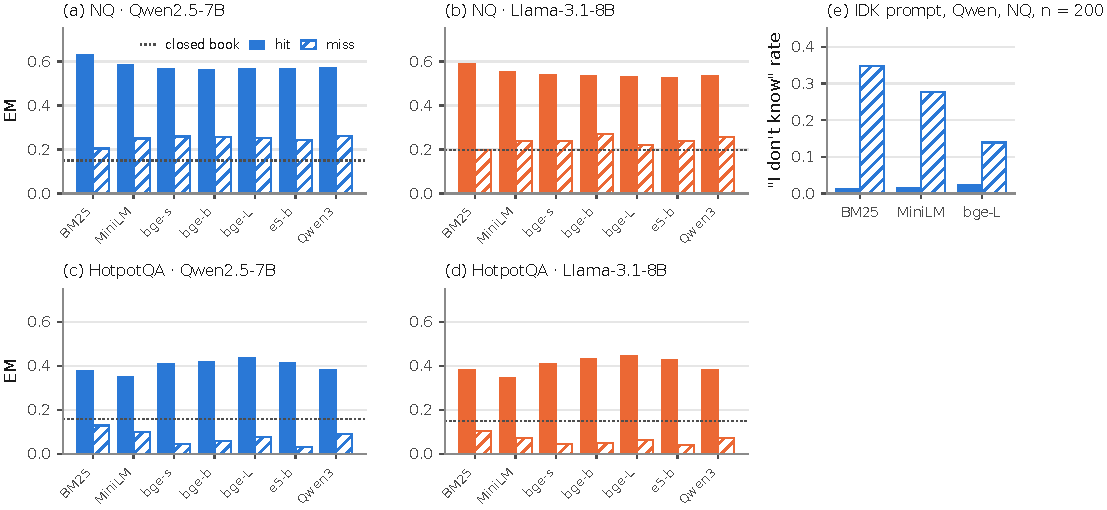
\includegraphics[width=\linewidth]{figs/fig10_error.pdf}
\caption{(a)--(d) Exact match given a hit (solid) and given a miss (hatched) at Hit@5, per reader--dataset cell; dotted line: closed-book EM. (e) Share of ``I don't know'' answers on hits and misses under the abstention prompt A3 (Phase~1, Qwen reader, NQ, 200 queries).}
\label{fig:error}
\end{figure}

\paragraph{Abstention prompt}
A Phase~1 check (Table~\ref{tab:idk}) is consistent with the reading that NQ ``misses'' often still contain usable evidence. When the prompt allowed ``I don't know'' (A3, Appendix~\ref{app:prompts}), the reader abstained mostly on misses: \ev{IDK.miss.R0} of BM25 misses, \ev{IDK.miss.R1} of MiniLM-L6 misses and \ev{IDK.miss.R4} of bge-large misses, against \ev{IDK.hit.R0} to \ev{IDK.hit.R4} of hits. Most misses were still answered. EM under A3 did not differ detectably from the main prompt (\ev{IDK.dem.R0}, \ev{IDK.dem.R1} and \ev{IDK.dem.R4}; $p\ge$ \ev{IDK.p.R4}).

\subsection{Encoder comparisons (RQ2)}\label{sec:res-encoders}
The P2 criterion was met on NQ and not met on HotpotQA (Table~\ref{tab:predictions}). On NQ, neither bge-large nor Qwen3-Embedding-0.6B differed detectably from e5-base-v2 in EM with either reader. On HotpotQA, bge-large gave higher EM than e5-base-v2 with both readers (\ev{P2.qhp.R4}, Holm-adjusted $p$ = \ev{P2.qhp.R4.p}; \ev{P2.lhp.R4}, $p$ = \ev{P2.lhp.R4.p}), in line with its higher Both@5. Qwen3-Embedding-0.6B gave lower EM than e5-base-v2 on HotpotQA (\ev{P2.qhp.R6}, $p$ = \ev{P2.qhp.R6.p}; \ev{P2.lhp.R6}, $p$ = \ev{P2.lhp.R6.p}). The registered pooled model over all four cells (Table~\ref{tab:gee}; \ev{GEE.rows} answers in \ev{GEE.clusters} query clusters) gave odds ratios of \ev{GEE.or.R4} \ev{GEE.ci.R4} for bge-large and \ev{GEE.or.R6} \ev{GEE.ci.R6} for Qwen3-Embedding-0.6B, each against e5-base-v2. This main-effects model assumes the same retriever effect on both datasets, and the data do not support that assumption: the retriever $\times$ dataset terms were jointly significant (Wald $\chi^2_{\ev{V4.gee.int.df}}$ = \ev{V4.gee.int.chi}, $p$ = \ev{V4.gee.int.p}), while retriever $\times$ reader terms were not ($p$ = \ev{V4.gee.rxr.p}). In the interaction model (post hoc), bge-large had an odds ratio of \ev{V4.or.R4.nq} \ev{V4.or.R4.nq.ci} on NQ and \ev{V4.or.R4.hp} \ev{V4.or.R4.hp.ci} on HotpotQA; Qwen3-Embedding-0.6B had \ev{V4.or.R6.nq} \ev{V4.or.R6.nq.ci} and \ev{V4.or.R6.hp} \ev{V4.or.R6.hp.ci}. The small pooled advantage of bge-large thus averages no detected effect on NQ with a gain on HotpotQA, in line with the per-cell tests. Both models mix the two study phases and are secondary.

\begin{table*}[t]
\centering
\small
\caption{GEE logistic models of EM over the four reader--dataset cells: odds ratios against e5-base-v2 [95\% CI].}
\label{tab:gee}
\begin{tabular}{lccc}
\toprule
 & Pooled (main effects) & \multicolumn{2}{c}{With retriever $\times$ dataset interaction} \\
\cmidrule(lr){3-4}
Contrast & both datasets & NQ & HotpotQA \\
\midrule
bge-large vs e5-base-v2 & 1.038 [1.001, 1.076] & 0.981 [0.936, 1.028] & 1.109 [1.049, 1.172] \\
Qwen3-Emb-0.6B vs e5-base-v2 & 0.909 [0.875, 0.943] & 0.952 [0.906, 1.001] & 0.859 [0.811, 0.909] \\
\bottomrule
\end{tabular}
\par\smallskip\parbox{\linewidth}{\footnotesize Pooled: EM $\sim$ retriever + dataset + reader (registered secondary model). Interaction model: EM $\sim$ retriever $\times$ dataset + reader (post hoc). Retriever $\times$ dataset: Wald $\chi^2_{6}$ = 179, $p$ = $5.2\times10^{-36}$; adding retriever $\times$ reader: $\chi^2_{6}$ = 5.0, $p$ = 0.55. Exchangeable working correlation (0.60) within query; 59,570 answers in 4,255 query clusters; empirical (sandwich) standard errors. All models converged without warnings.}
\end{table*}


\subsection{Context choices (RQ3)}\label{sec:res-context}
\paragraph{Number of passages}
Table~\ref{tab:topk} and Fig.~\ref{fig:topk} show EM for $k\in\{1,3,5,10\}$ with Qwen on NQ. One passage gave lower EM than five for every retriever (P4 criterion met; differences from \ev{K1.R0} for BM25 to \ev{K1.R5} for e5-base-v2, all Holm-adjusted $p<0.001$). From five to ten passages, EM rose for six retrievers and stayed flat for e5-base-v2 (\ev{TK.R5.k5} and \ev{TK.R5.k10}). The gap between retrievers shrank with $k$: at $k=10$ all dense encoders gave EM between \ev{TK.R1.k10} and \ev{TK.R4.k10}. In an exploratory check (Table~\ref{tab:transferk}), we matched Hit@$k$ to the $k$ passages the reader saw. The transfer ratio then fell with $k$; for bge-large it was \ev{TKT.R4.k1} \ev{TKT.R4.k1.ci} at $k=1$, \ev{TKT.R4.k3} at $k=3$, \ev{TKT.R4.k5} at $k=5$ and \ev{TKT.R4.k10} \ev{TKT.R4.k10.ci} at $k=10$. The NQ ratios of Section~\ref{sec:res-transfer} therefore describe $k=5$ only. More passages also cost more reading: the mean prompt grew from \ev{TOK.R4_k1} tokens at $k=1$ to \ev{TOK.R4_k5} at $k=5$ and \ev{TOK.R4_k10} at $k=10$ for bge-large. In a second exploratory comparison, bge-large with one passage gave higher EM than BM25 with ten passages (\ev{X41.diff} \ev{X41.ci}; exact McNemar $p$ = \ev{X41.p}, uncorrected).

\begin{figure}[t]
\centering
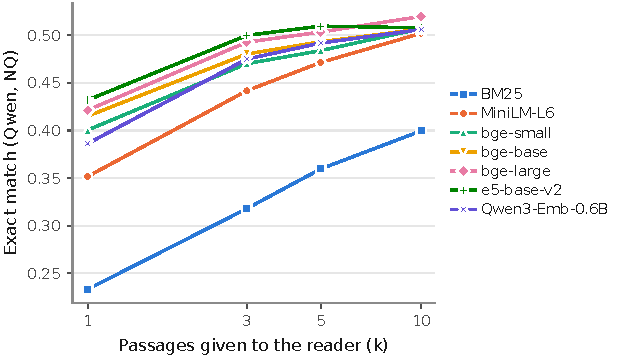
\includegraphics[width=0.85\linewidth]{figs/fig3_topk.pdf}
\caption{Exact match by number of passages $k$, Qwen reader on NQ (2,255 queries).}
\label{fig:topk}
\end{figure}

\paragraph{Passage composition and position}
Table~\ref{tab:mechanism} and Fig.~\ref{fig:mechanism} give the controlled context test on 500 NQ questions. With the gold passage at position 1, four top-ranked non-gold BM25 passages gave EM \ev{MC.M1}, and four random passages gave \ev{MC.MR}: a drop of \ev{P5.abs} (exact McNemar $p$ = \ev{P5.p}; P5 criterion met). Adding four random passages to the gold passage changed EM by no detectable amount: gold at position 1 plus four random passages gave \ev{MC.MR}, and the gold passage alone gave \ev{MC.MG} (difference \ev{V4.mrmg.diff}, 95\% CI \ev{V4.mrmg.ci}; $p$ = \ev{MG.p}). No equivalence margin was registered, so this interval is not evidence that random passages have no effect; it only bounds the effect in this sample of 500 questions. Under the answer-string rule, at least one hard negative contained an answer for \ev{V6.o8.n} of the 500 questions (\ev{V6.o8.share}, Wilson interval \ev{V6.o8.wilson}). On the \ev{V6.o8.clean.n} questions without such a passage, the drop was larger: EM \ev{V6.o8.clean.M1} with hard negatives against \ev{V6.o8.clean.MR} with random passages (\ev{V6.o8.clean.diff}, 95\% CI \ev{V6.o8.clean.ci}; $p$ \ev{V6.o8.clean.p}). On the other questions the two contexts gave \ev{V6.o8.ans.M1} and \ev{V6.o8.ans.MR} (not pre-specified). Answer-bearing hard negatives therefore made the registered P5 effect smaller, not larger. The position of the gold passage among the hard negatives showed no detectable effect (EM \ev{MC.M1}, \ev{MC.M3} and \ev{MC.M5} at positions 1, 3 and 5; all Holm-adjusted $p\ge$ \ev{P6.M1M3.p}; P6 criterion not met).

\begin{figure}[t]
\centering
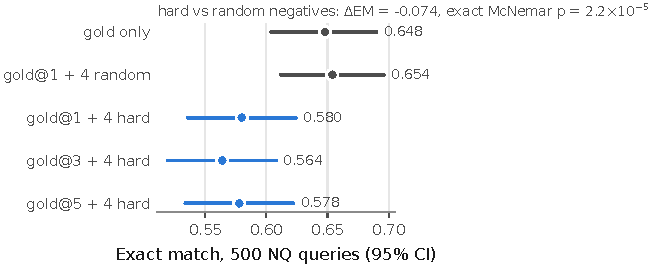
\includegraphics[width=0.75\linewidth]{figs/fig4_mechanism.pdf}
\caption{Exact match for five controlled contexts of five passages (Qwen reader, 500 NQ generation queries) with 95\% bootstrap intervals.}
\label{fig:mechanism}
\end{figure}

\begin{table}[t]
\centering
\small
\caption{Exact match by number of passages $k$ (Qwen reader, NQ, 2,255 queries).}
\label{tab:topk}
\begin{tabular}{lrrrrrr}
\toprule
Retriever & $k{=}1$ & $k{=}3$ & $k{=}5$ & $k{=}10$ & $\Delta_{1-5}$ & $p_\text{Holm}$ \\
\midrule
BM25 & 0.233 & 0.318 & 0.360 & 0.400 & $-$0.126 & $<$0.001 \\
MiniLM-L6 & 0.352 & 0.442 & 0.471 & 0.502 & $-$0.120 & $<$0.001 \\
bge-small & 0.400 & 0.470 & 0.484 & 0.507 & $-$0.083 & $<$0.001 \\
bge-base & 0.415 & 0.480 & 0.493 & 0.506 & $-$0.078 & $<$0.001 \\
bge-large & 0.421 & 0.493 & 0.503 & 0.520 & $-$0.082 & $<$0.001 \\
e5-base-v2 & 0.432 & 0.500 & 0.510 & 0.508 & $-$0.078 & $<$0.001 \\
Qwen3-Emb-0.6B & 0.386 & 0.475 & 0.492 & 0.506 & $-$0.106 & $<$0.001 \\
\bottomrule
\end{tabular}
\par\smallskip\parbox{\linewidth}{\footnotesize Exact McNemar test of $k{=}1$ vs $k{=}5$, Holm over seven retrievers.}
\end{table}

\begin{table}[t]
\centering
\small
\caption{Distraction and position tests (Qwen reader, 500 NQ generation queries).}
\label{tab:mechanism}
\begin{tabular}{lccc}
\toprule
Context (5 passages) & EM [95\% CI] & F1 & AC \\
\midrule
Gold only & 0.648 [0.604, 0.690] & 0.772 & 0.770 \\
Gold@1 + 4 random & 0.654 [0.612, 0.696] & 0.777 & 0.764 \\
Gold@1 + 4 hard & 0.580 [0.536, 0.624] & 0.696 & 0.686 \\
Gold@3 + 4 hard & 0.564 [0.520, 0.608] & 0.684 & 0.672 \\
Gold@5 + 4 hard & 0.578 [0.534, 0.622] & 0.698 & 0.682 \\
\bottomrule
\end{tabular}
\par\smallskip\parbox{\linewidth}{\footnotesize Hard vs random negatives: $\Delta$EM = $-$0.074, exact McNemar $p$ = $2.2\times10^{-{}5}$. Position: no pair differs after Holm.}
\end{table}


\paragraph{Reranking}
The cross-encoder raised the Hit@5 and EM of BM25 and lowered the Hit@5 of e5-base-v2 (Table~\ref{tab:reranker}). On the NQ generation queries, reranking the BM25 top 50 raised Hit@5 by \ev{RR.X0_vs_R0.hit} and EM by \ev{RR.X0_vs_R0.em} (both $p<0.001$). Reranking the e5-base-v2 top 50 changed Hit@5 by \ev{RR.X5_vs_R5.hit} ($p$ = \ev{RR.X5_vs_R5.hit.p}); for EM the change was \ev{RR.X5_vs_R5.em} ($p$ = \ev{RR.X5_vs_R5.em.p}), and no difference was detected. Reranking cost a median of \ev{RR.lat.R0} to \ev{RR.lat.R5}~ms per query on a T4. These results come from one reranker at one depth.

\begin{table}[t]
\centering
\small
\caption{Cross-encoder reranking (bge-reranker-base, top 50) on NQ.}
\label{tab:reranker}
\begin{tabular}{lcccc}
\toprule
System & Hit@5 & nDCG@10 & EM & ms/query \\
\midrule
BM25 & 0.373 & 0.284 & 0.360 & -- \\
BM25 + reranker & 0.658 & 0.542 & 0.456 & 208 \\
e5-base-v2 & 0.817 & 0.665 & 0.510 & -- \\
e5-base-v2 + reranker & 0.742 & 0.601 & 0.494 & 249 \\
\bottomrule
\end{tabular}
\par\smallskip\parbox{\linewidth}{\footnotesize Retrieval on all 3,452 judged queries; EM on the 2,255 generation queries (Qwen). Latency: median per query, 50 pairs, one T4.}
\end{table}


\subsection{Retrieval-stage cost and checks of the setup (RQ4)}\label{sec:res-cost}
\paragraph{Encoding cost}
Table~\ref{tab:cost} gives the measured retrieval-stage cost; reader cost was not part of this measurement. Throughput fell from \ev{E7.tp.R1} passages per second for MiniLM-L6 to \ev{E7.tp.R6} for Qwen3-Embedding-0.6B, a factor of \ev{E7.ratio.R1R6}. e5-base-v2 encoded \ev{E7.ratio.R5R4} times faster than bge-large. The five repetitions varied little (Table~\ref{tab:cost}): no two encoders had overlapping throughput ranges. The closest pair, bge-base and e5-base-v2, share the same architecture size, and bge-base was \ev{V4.tp.R3R5} faster at the median. Query encoding took \ev{E7.lat.R1} to \ev{E7.lat.R6}~ms per query; BM25 took \ev{E7.lat.R0}~ms on the CPU. Fig.~\ref{fig:cost} relates throughput to EM averaged over the four cells. bge-large had the highest average EM (\ev{EMBAR.R4}), bge-base and e5-base-v2 followed at \ev{EMBAR.R5} with \ev{E7.ratio.R5R4} times its throughput, and Qwen3-Embedding-0.6B (\ev{EMBAR.R6}) was both the slowest and below bge-small (\ev{EMBAR.R2}).

\begin{figure}[t]
\centering
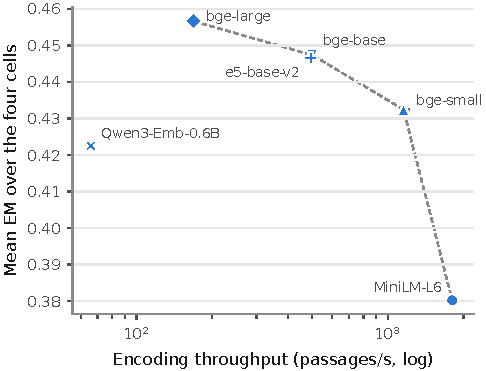
\includegraphics[width=0.6\linewidth]{figs/fig5_cost_quality.pdf}
\caption{Encoding throughput on one T4 GPU (median of five repetitions, log scale) against EM averaged over the four reader--dataset cells. The dashed line joins encoders that no other encoder beats on both axes.}
\label{fig:cost}
\end{figure}

\begin{table}[t]
\centering
\small
\caption{Encoding cost on one Tesla T4, median (range) over five repetitions.}
\label{tab:cost}
\begin{tabular}{lrrcc}
\toprule
Encoder & Params (M) & Dim & Passages/s & Query ms \\
\midrule
MiniLM-L6 & 23 & 384 & 1807 (1768--1863) & 6.0 (6.0--6.1) \\
bge-small & 33 & 384 & 1155 (1136--1207) & 10.3 (10.1--10.3) \\
bge-base & 109 & 768 & 502 (501--503) & 10.0 (9.9--10.1) \\
e5-base-v2 & 109 & 768 & 493 (491--496) & 10.0 (9.9--10.1) \\
bge-large & 335 & 1024 & 168 (168--169) & 18.3 (18.3--18.6) \\
Qwen3-Emb-0.6B & 596 & 1024 & 66 (66--66) & 52.2 (51.8--54.9) \\
\bottomrule
\end{tabular}
\par\smallskip\parbox{\linewidth}{\footnotesize BM25 batch-1 query latency on CPU: 25.7 ms (23.7--27.7).}
\end{table}


\paragraph{CPU deployment} Phase~1 also measured single-query latency with encoding and exact search on the CPU, index size and full sub-corpus encoding time (single measurements). These operational details, with the CPU quality--latency frontier, are in Appendix~\ref{app:deploy}.

\paragraph{Approximate search}
HNSW search kept the exact top five almost unchanged (Table~\ref{tab:hnsw}). At efSearch 128, HNSW returned at least \ev{V5.hnsw.ov5.min128} of the exact top five and \ev{V5.hnsw.ov100.min128} of the exact top 100 (mean shares over all 3,452 judged queries), Hit@5 changed by at most \ev{E6.dhitabs.max}, and the median query latency on the CPU fell from \ev{E6.lat.exact.R1}--\ev{E6.lat.exact.R5}~ms to \ev{E6.lat.ef128.R1}--\ev{E6.lat.ef128.R5}~ms. We did not run the readers on HNSW results, so this check covers retrieval and latency only.

\begin{table*}[t]
\centering
\footnotesize
\caption{Approximate search (HNSW, $M{=}32$, efConstruction 200) against exact search on the NQ sub-corpus, CPU, all 3,452 judged NQ queries.}
\label{tab:hnsw}
\begin{tabular}{lcccccccccc}
\toprule
& \multicolumn{2}{c}{Exact} & \multicolumn{4}{c}{HNSW efSearch 64} & \multicolumn{4}{c}{HNSW efSearch 128} \\ \cmidrule(lr){2-3}\cmidrule(lr){4-7}\cmidrule(lr){8-11} Encoder & Hit@5 & ms & Ov@5 & Ov@100 & Hit@5 & ms & Ov@5 & Ov@100 & Hit@5 & ms \\
\midrule
MiniLM-L6 & 0.673 & 35.9 & 0.998 & 0.946 & 0.672 & 0.50 & 0.999 & 0.984 & 0.673 & 0.84 \\
bge-small & 0.729 & 36.3 & 0.992 & 0.904 & 0.726 & 0.49 & 0.996 & 0.964 & 0.727 & 0.89 \\
e5-base-v2 & 0.817 & 77.7 & 0.995 & 0.915 & 0.815 & 0.80 & 0.997 & 0.970 & 0.817 & 1.45 \\
\bottomrule
\end{tabular}
\par\smallskip\parbox{\linewidth}{\footnotesize Ov@5 / Ov@100: mean share of the exact top 5 / top 100 that HNSW also returns. Hit@5 here is over all judged queries, not the 2,255 generation queries. ms: median batch-1 query latency on 4 vCPUs. No reader was run on HNSW results.}
\end{table*}


\paragraph{Sub-corpus versus full corpus}
On the full NQ corpus the four tested retrievers kept their nDCG@10 order (Kendall's $\tau$ = \ev{E9.tau}; P3 criterion met; Table~\ref{tab:fullcorpus} and Fig.~\ref{fig:fullcorpus}). The dense retrievers lost \ev{E9.dropabs.R2} to \ev{E9.dropabs.R1} in nDCG@10, and BM25 lost almost nothing (\ev{E9.dropabs.R0}). The sub-corpus therefore inflates absolute dense scores but not the order of these four retrievers. The drops also agree with the bias that the construction implies: the sub-corpus keeps BM25's own top-ranked passages for every judged query but not those of the dense encoders, so it favours the dense encoders relative to BM25. Section~\ref{sec:res-full} gives the readers on full-corpus retrieval; HotpotQA was not run on its full corpus.

\begin{figure}[t]
\centering
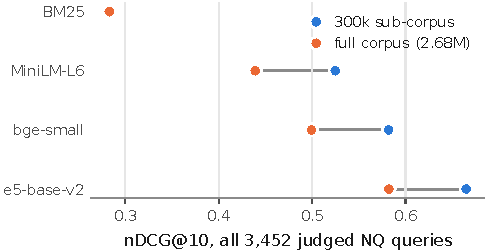
\includegraphics[width=0.6\linewidth]{figs/fig6_full_corpus.pdf}
\caption{nDCG@10 on the 300,000-passage sub-corpus and on the full NQ corpus (all 3,452 judged queries).}
\label{fig:fullcorpus}
\end{figure}

\begin{table}[t]
\centering
\small
\caption{Sub-corpus (300k) vs full NQ corpus (2.68M), all 3,452 judged queries.}
\label{tab:fullcorpus}
\begin{tabular}{lcccc}
\toprule
Retriever & nDCG@10 sub & nDCG@10 full & Hit@5 sub & Hit@5 full \\
\midrule
BM25 & 0.284 & 0.283 & 0.373 & 0.373 \\
MiniLM-L6 & 0.525 & 0.439 & 0.673 & 0.571 \\
bge-small & 0.582 & 0.499 & 0.729 & 0.630 \\
e5-base-v2 & 0.665 & 0.582 & 0.817 & 0.727 \\
\bottomrule
\end{tabular}
\par\smallskip\parbox{\linewidth}{\footnotesize Kendall's $\tau$ between the two orderings = 1.00.}
\end{table}


\subsection{LLM judge validation}\label{sec:res-judge}
The LLM judge agreed poorly with the author's labels (Table~\ref{tab:judge}). Cohen's $\kappa$ was \ev{JA.kappa} \ev{JA.ci}, with raw agreement \ev{JA.raw}. Weighted to the population, the judge labelled \ev{JA.jrate} of answers as supported, against \ev{JA.hrate} for the author, and its precision for the label supported was \ev{JA.prec}. Under the registered rule ($\kappa<0.2$) we excluded the judge's faithfulness labels from all conclusions. For completeness, Table~\ref{tab:judgerates} in the appendix lists the share of answers the judge labelled as supported, and Appendix~\ref{app:judge} gives the judge prompt and the annotation instructions.

\begin{table}[t]
\centering
\small
\caption{Agreement between the author's labels and the LLM judge on 200 stratified items.}
\label{tab:judge}
\begin{tabular}{lcc}
\toprule
& Judge SUPPORTED & Judge NOT\_SUPPORTED \\
\midrule
Human SUPPORTED & 65 & 50 \\
Human NOT\_SUPPORTED & 37 & 48 \\
\bottomrule
\end{tabular}
\par\smallskip\parbox{\linewidth}{\footnotesize Cohen's $\kappa$ = 0.127 [$-$0.006, 0.261]; raw agreement 0.565. Under the pre-registered rule ($\kappa<0.2$) the judge results are excluded from the conclusions.}
\end{table}


\subsection{Summary of the predictions}
Table~\ref{tab:predictions} lists all eight registered criteria. P3, P4, P5, P7 and P8 were met. P1 was not met in one of three new cells (an upper bound of 1.000 or more), P2 was not met in either HotpotQA cell, and P6 was not met. Where a verdict is not confirmatory, the table marks it.

\begin{table*}[t]
\centering
\small
\caption{Registered predictions: whether each stated criterion was met.}
\label{tab:predictions}
\begin{tabular}{lllp{0.55\linewidth}}
\toprule
ID & Scope & Criterion & Evidence \\
\midrule
P1 & NQ, Qwen$^\dagger$ & met & 5 dense-encoder ratios; largest upper bound 0.455 (Qwen3-Emb-0.6B) \\
P1 & NQ, Llama & met & 5 dense-encoder ratios; largest upper bound 0.427 (bge-small) \\
P1 & HotpotQA, Qwen & met & 5 dense-encoder ratios; largest upper bound 0.996 (bge-large) \\
P1 & HotpotQA, Llama & \textbf{not met} & 5 dense-encoder ratios; largest upper bound 1.096 (bge-large) \\
P2 & NQ, Qwen$^\dagger$ & met & bge-large $-$ e5: $-$0.006 ($p_\text{Holm}$ 1.000); Qwen3-Emb-0.6B $-$ e5: $-$0.018 ($p_\text{Holm}$ 0.271) \\
P2 & NQ, Llama & met & bge-large $-$ e5: $-$0.004 ($p_\text{Holm}$ 1.000); Qwen3-Emb-0.6B $-$ e5: $-$0.007 ($p_\text{Holm}$ 1.000) \\
P2 & HotpotQA, Qwen & \textbf{not met} & bge-large $-$ e5: +0.028 ($p_\text{Holm}$ 0.005); Qwen3-Emb-0.6B $-$ e5: $-$0.030 ($p_\text{Holm}$ 0.003) \\
P2 & HotpotQA, Llama & \textbf{not met} & bge-large $-$ e5: +0.022 ($p_\text{Holm}$ 0.040); Qwen3-Emb-0.6B $-$ e5: $-$0.042 ($p_\text{Holm}$ $<$0.001) \\
P3 & NQ, 4 retrievers & met & Kendall's $\tau$ = 1.00 (retrieval only) \\
P4 & NQ, Qwen & met & $k{=}1$ below $k{=}5$ for all 7 retrievers$^\ddagger$; $\Delta$EM $-$0.126 to $-$0.078; all $p_\text{Holm}$ $<$0.001 \\
P5 & NQ, Qwen, 500 q. & met & hard vs random negatives: $\Delta$EM $-$0.074, $p$ $<$0.001 \\
P6 & NQ, Qwen, 500 q. & \textbf{not met} & gold at position 1/3/5: largest $|\Delta$EM$|$ 0.016; smallest $p_\text{Holm}$ 0.94 \\
\bottomrule
\end{tabular}
\par\smallskip\parbox{\linewidth}{\footnotesize P1: every reportable EM transfer ratio of a dense encoder has an upper 95\% bound below 1 (unrounded; a bound of exactly 1.000 does not meet it). P2: no Holm-significant EM gain of bge-large or Qwen3-Emb-0.6B over e5-base-v2. P3: the full corpus keeps the nDCG@10 ordering. P4: EM at $k{=}1$ below $k{=}5$. P5: hard negatives lower EM. P6: gold position changes EM. $^\dagger$Not confirmatory: observed in Phase 1, before registration. $^\ddagger$Confirmatory for bge-small, bge-base, e5-base-v2 and Qwen3-Emb-0.6B only. The v0.3 analysis code also counted BM25 in the NQ P1 checks (six ratios); the registered criterion covers dense encoders, and the verdict is the same either way.}
\end{table*}

